% This is LLNCS.DEM the demonstration file of
% the LaTeX macro package from Springer-Verlag
% for Lecture Notes in Computer Science,
% version 2.4 for LaTeX2e as of 16. April 2010
%
\documentclass{llncs}
\usepackage{graphicx}
\usepackage{wrapfig}
\usepackage{makeidx}  % allows for indexgeneration
\usepackage{bibspacing}
\usepackage{fancyvrb}
\setlength{\bibspacing}{\baselineskip}
\usepackage[tight,footnotesize]{subfigure}

\newcommand{\mySection}[1]{\vspace{-5pt}\section{\hskip -1em.~~#1}\vspace{-10pt}}
\newcommand{\mySubSection}[1]{\vspace{-5pt}\subsection{\hskip -1em.~~#1}\vspace{-10pt}}
\newcommand{\mySubSubSection}[1]{\vspace{-5pt}\subsubsection{\hskip -1em.~~#1}\vspace{-5pt}}
\newcommand{\tableref}[1]{Table~\ref{tab:#1}}
\newcommand{\figref}[1]{Fig.~\ref{fig:#1}}
\newcommand{\Hao}[1]{$\clubsuit$\footnote{HAO: #1}}

%\setlength{\textheight}{22cm}
%\setlength{\textwidth}{12cm}
%%%\setlength{\columnsep}{0.2in}
%%%\setlength{\botmargin}{-1.0in}
%%\setlength{\headheight}{+0.5in}
%\setlength{\headsep}{-0.2in}
%%\setlength{\parindent}{1pc}
%\setlength{\oddsidemargin}{+.4in}
%\setlength{\evensidemargin}{+.4in}

\begin{document}
%
\frontmatter          % for the preliminaries
%
\pagestyle{headings}  % switches on printing of running heads
%\addtocmark{Hamiltonian Mechanics} % additional mark in the TOC
%
          % start of the contributions
%
%\title{A Matlab Toolbox for EP Heart Modeling}
\title{Requirement-Guided Model Refinement}
%\titlerunning{Pacemaker Verification}  % abbreviated title (for running head)
\author{Zhihao Jiang}\vspace{-10pt}
\authorrunning{Jiang et al.} % abbreviated author list (for running head)
\institute{University of Pennsylvania, Philadelphia PA, USA\footnote{This document serves as the final report for Zhihao Jiang's internship at Mathworks during Summer 2014, under supervision of Pieter Mosterman from Mathworks and Prof. Rahul Mangharam from University of Pennsylvania.}}

\maketitle              % typeset the title of the contribution
\vspace{-10pt}
% \begin{abstract}
% In this report I will present a matlab toolbox 
% \end{abstract}

% \begin{figure*}
% \centering

% 		\subfigure {
% 				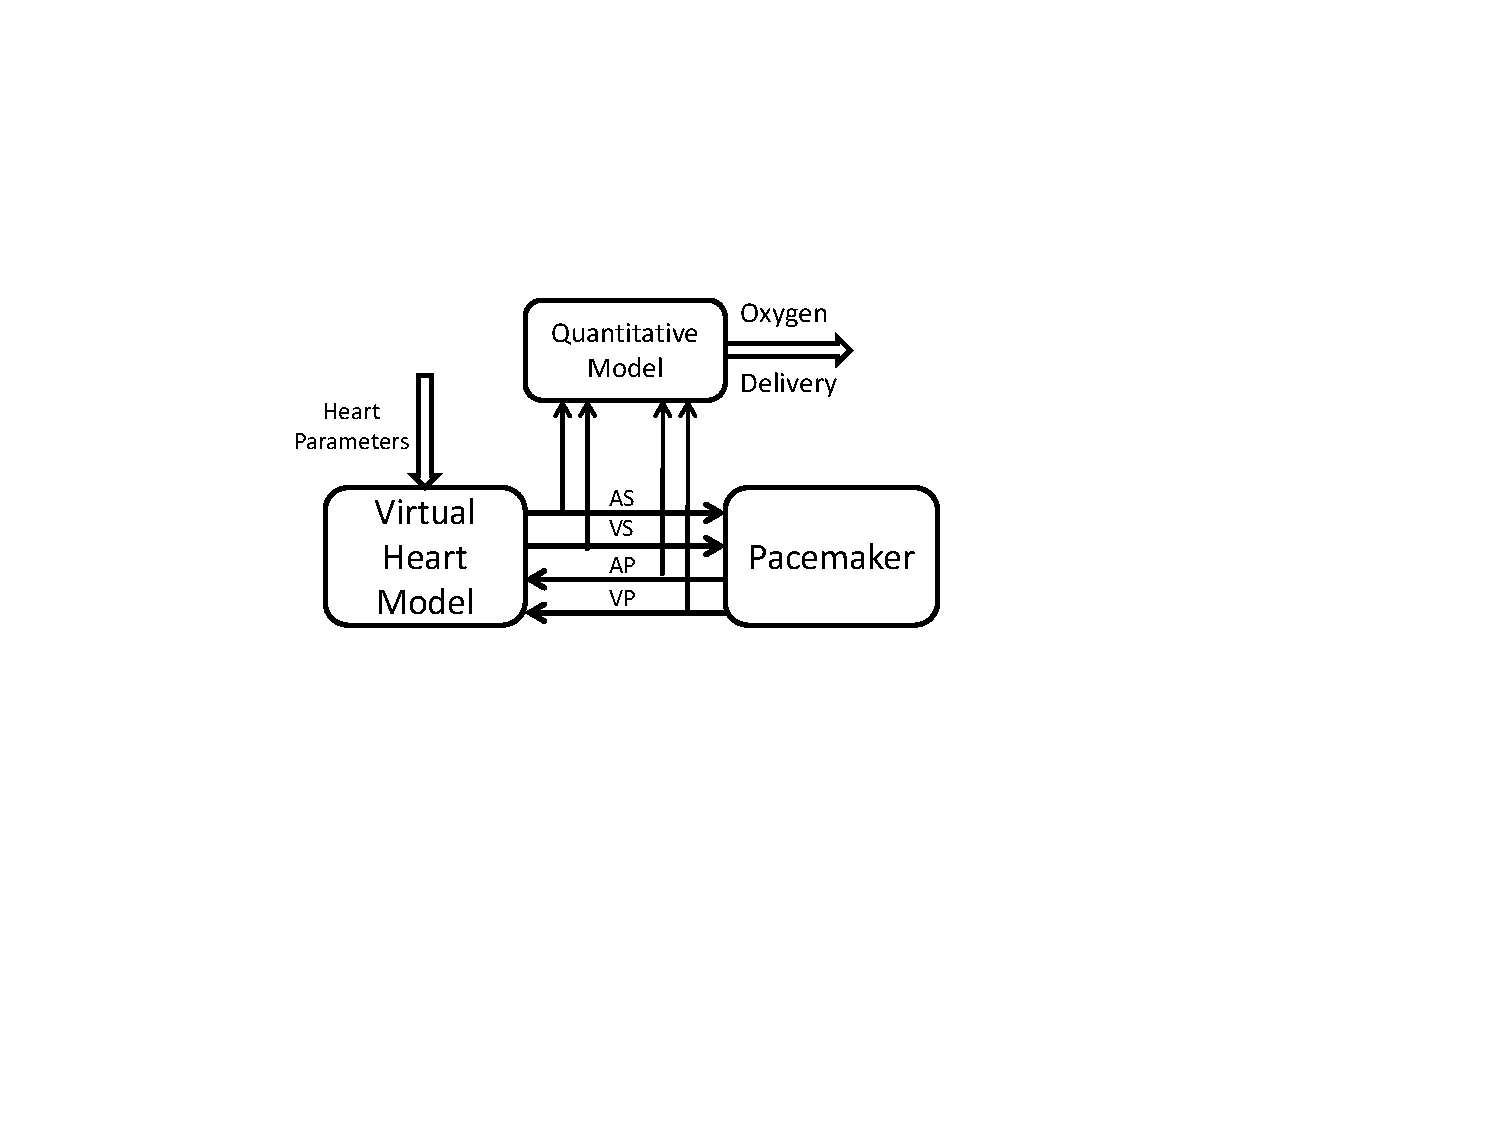
\includegraphics[width=0.45\textwidth]{figs/overall.pdf}
% 				\label{fig:overall}
% 		} 
% 		\subfigure {	
% 			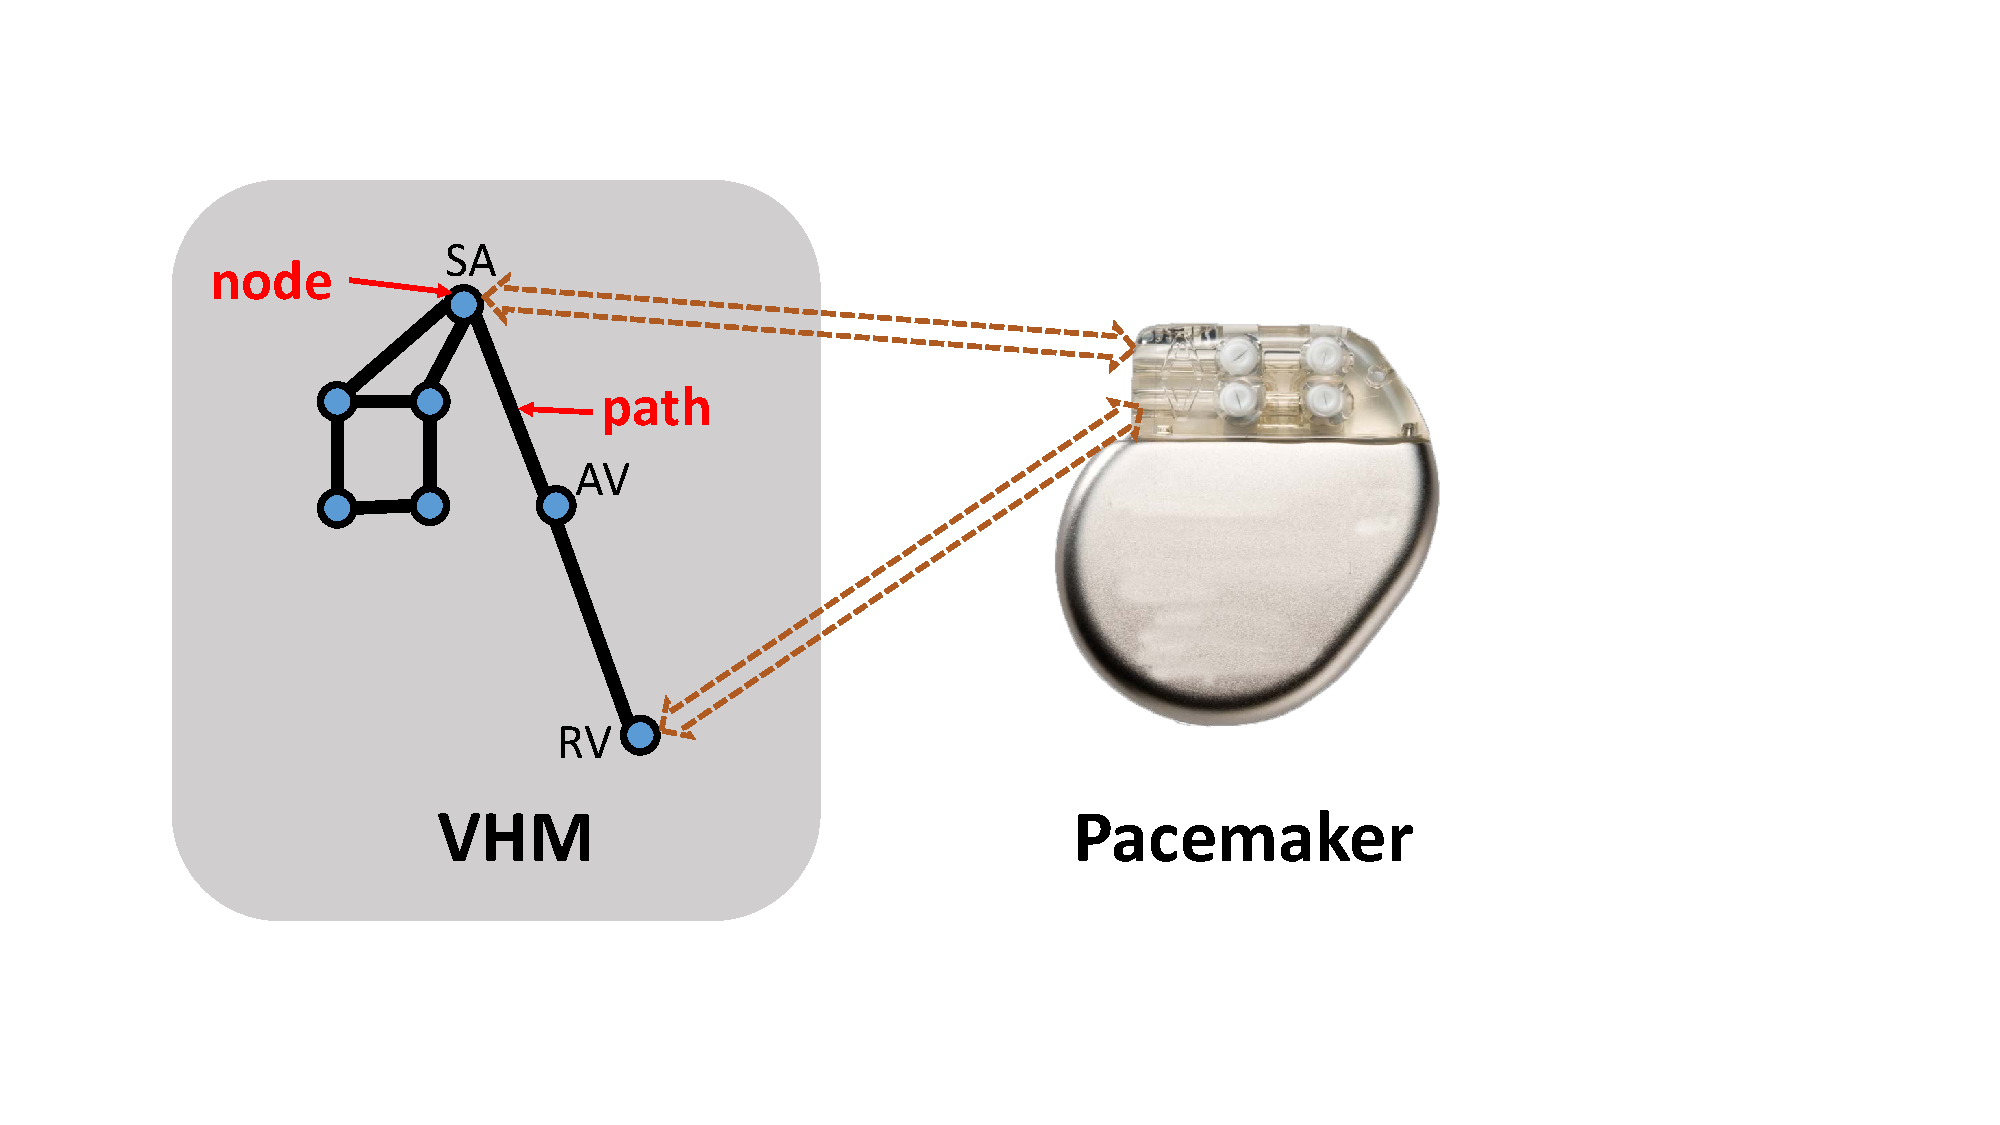
\includegraphics[width=0.45\textwidth]{figs/layout.pdf}
% 			\label{fig:VHM}
% 		}
        
%         	\caption{(a) System layout. (b) A sample closed-loop system}
% \end{figure*}

\section{Introduction}
Medical device is a typical Cyber-Physical System and ensuring the safety and efficacy of the device requires closed-loop verification. Currently closed-loop verifications of medical devices are performed in the form of clinical trials in which the devices are tested on the patients. Using clinical trials as closed-loop verification has several problems:
\begin{itemize}
	\item The cost of clinical trials are high
    \item Due to the cost, the scale of the clinical trials cannot be large, thus affecting patient generality and the effectiveness of the trials.
    \item It is the last step of the design process thus discovering a bug at this stage is very costly to fix.
\end{itemize}
In \cite{VHM_proc} we addressed the problems above by proposing a model-based design framework to enable closed-loop verification earlier in the design stage. The increased confidence in safety and efficacy of the device can potentially reduce the scale of the clinical trials, thus reduce cost.

The biggest challenge for closed-loop evaluation is to bridge the domain knowledge gap between the domain experts and software developers. These domain knowledge are two folds:
\begin{enumerate}
	\item How the physical plant works?
    \item Evaluation of the well-being of the patient (Performance)
\end{enumerate}
From tool developer's perspective, both of the aspects need to be addressed.
\subsection{How the physical plant works?}
The first aspect can be addressed by developing appropriate model(s) of the physical plant. The word "appropriate" means two things:
\begin{itemize}
	\item The model is validated, such that it captures the correct input-output of the system that it models.
    \item The model has the correct level of abstraction, such that it has to be complex enough to model the required details of the patients' condition, and at the same time avoid over-complexity.
\end{itemize}

In \cite{VHM_proc} we developed the Virtual Heart Model (VHM), which is an electrophysiological heart model structure that captures the timing behaviors of the electrical conduction system of the human heart. The model structure can be used to represent different patient conditions and those conditions are validated by the physicians. 

In \cite{sttt13}, we formally defined a series of heart models using the VHM structure. The heart models are at different abstraction levels and can be used for model checking of pacemaker software. We also adapted the Counter-Example Guided Abstraction and Refinement (CEGAR) framework \cite{cegar} to select the most appropriate model during model checking.

\subsection{Evaluation of the well-being of the patient (Performance)}
Having the models for the physical plant is important, thus this alone is not enough to bridge the gap between domain expert and software developers. These additional domain knowledge lies mostly in:
\begin{itemize}
	\item The requirements specified by the domain experts to evaluate the safety and efficacy of the device.
    \item Assumptions made during heart model abstractions
\end{itemize}
The connection between these two aspects and the heart models are not well formalized, which significantly limiting the ability of the software developers to use the heart models. 

In this project, we propose a Matlab toolbox for EP heart modeling to address the problem above during pacemaker software design. We formalized the abstraction rules and their effects on the model behaviors. Each heart model documents all the rules that were applied and all observable behaviors. These information can be used to 1) validate the model and 2) evaluate whether the model has enough information to express the heart conditions in the requirement. 

This report is arranged as follow. Section 2 introduces the observable behaviors of the heart. Section 3 formalizes the abstraction rules and their effects on the heart behaviors. Section 4 introduces the heart structure and validation. Section 5 introduces the requirements and how to use heart behaviors to detemine whether a heart model can be used to verify certain requirement.

% \begin{figure}[!t]
% 		\centering
% 		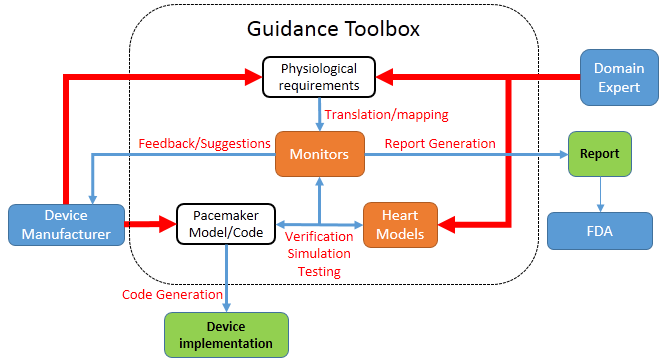
\includegraphics[width=0.8\textwidth]{figs/overall.png}
% 		%\vspace{-5pt}
% 		\caption{\small Overall Structure of the Toolbox}
% 		  %\vspace{-15pt}
% 		\label{fig:overall}
% \end{figure}
\section{Observable Behaviors of The Heart}
The observable EP heart behaviors are local depolarizations that can be recorded by placing electrodes against the inner heart wall. With these recordings, the physicians developed their own perspective of describing heart behaviors in terms of generation and conduction of depolarizations throughout the heart. In terms of modeling, the behaviors are state transitions of the model.%The pacemaker has only two leads into the heart, thus offering only two observable points for local depolarizations.

The following are the most fundamental behaviors to describe the behavior of the heart.
\begin{itemize}
	\item Self-activation (self):increase the number of activations
    \item Conduction (cond): maintain the number of activations %\Hao{Need to work on detail of this}
    \item Refractory Blocking (block): reduce the number of activations
    \item External Pacing (pace): increase the number of activations

\end{itemize}

We name the behavior of depolarization of certain heart tissue \emph{activation (act)}. It can be triggered by both \emph{self-activation} and \emph{conduction}. Ideally one activation generated either by self-activation or pacing will activate all the activatable tissue in the heart \textbf{once}.
\begin{figure}[!t]
		\centering
		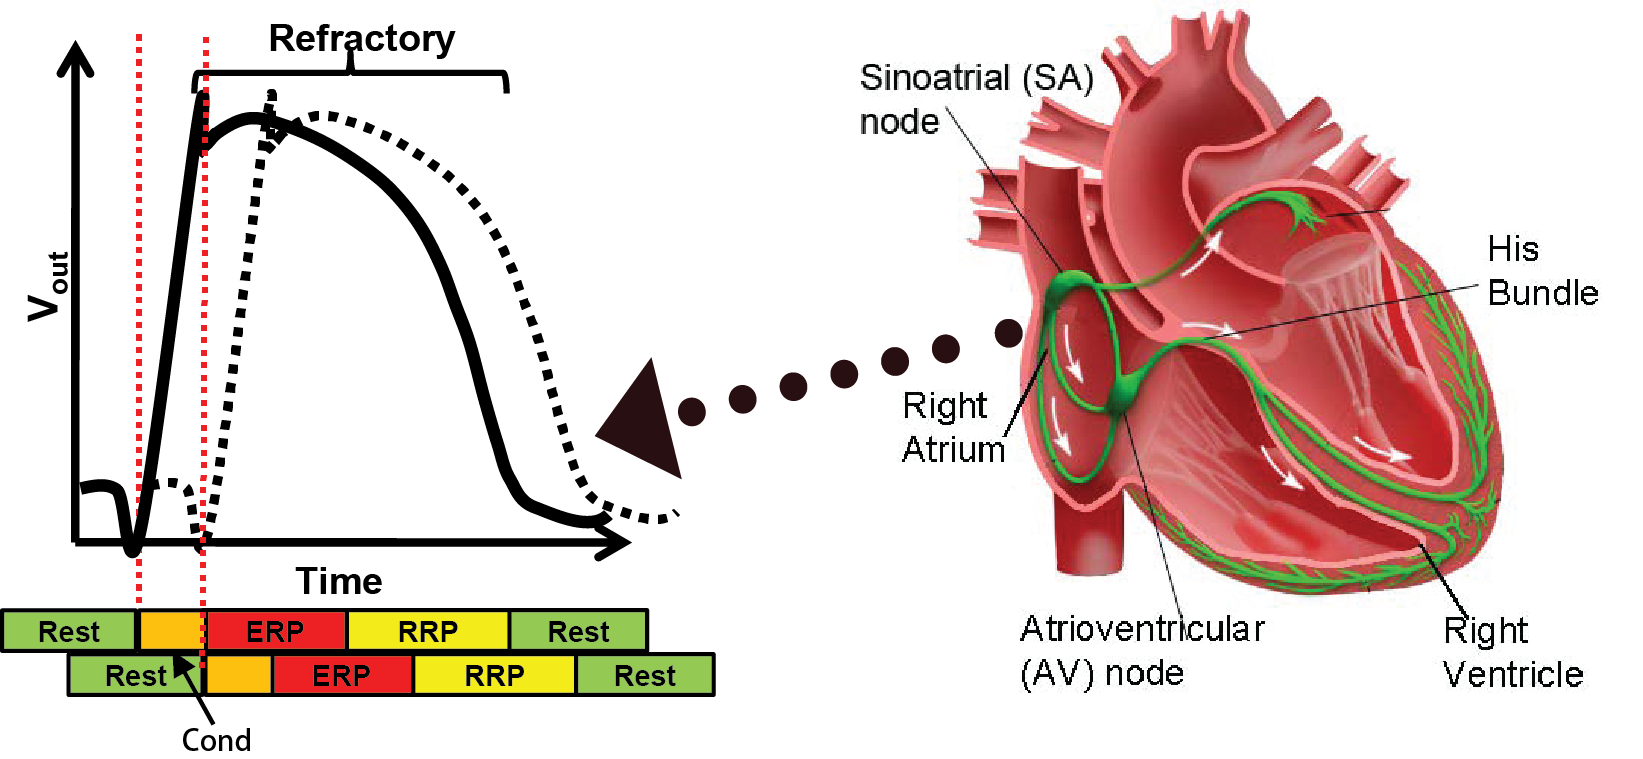
\includegraphics[width=0.8\textwidth]{figs/basic.png}
		%\vspace{-5pt}
		\caption{\small Heart Model Abstractions}
		  %\vspace{-15pt}
		\label{fig:abs}
\end{figure}
First there are identified structures within the electrical conduction system of the heart. Without forming a circle in the heart, the self-depolarization always happens in the \emph{SA node ($SA$)}. After depolarizing the whole atria, the depolarization signal reaches the \emph{AV node ($AV$)}. Then the signal travels through the \emph{His Bundle (His)} and depolarize the whole ventricle, including the \emph{Right Ventricular Apex (RVA)} through the \emph{Pukinje Fibers (Puk)}. 

Let $S$ be the set of structures and $B$ be the set of behaviors. We represent the behavior associated with a structure $s\in S$ using $s.b$. 

So we have the following behaviors: \textsf{SA.self}, \textsf{SA.block},  \textsf{SA\_AV.cond}, \textsf{AV.block}, \textsf{His.cond}, \textsf{His.block}, \textsf{Puk.cond}, \textsf{Puk.block}, \textsf{RVA.block}. Some tissue in the left atrium and the ventricles can self-depolarize prematurely. They are called \emph{Premature Atrial Contraction (PAC)} and \emph{Premature Ventricular Contraction (PVC)} respectively. So we have two more behavior: \textsf{PAC.self} and \textsf{PVC.self}. A typical heart cycle can be represented by a sequence of behaviors: \textsf{SA.self$\rightarrow$SA\_AV.cond $\rightarrow$ His.cond$\rightarrow$Puk.cond$\rightarrow$Vent.act}

\section{Abstraction Rules for the Heart}
Abstraction rules are based on both domain knowledge and reasoning. The rules may have dependencies among each other, and for rules that are independent of each other, applying them in different order on a heart model will yield the same result. 

In the next sub-section I will introduce the abstraction rules that we use for the toolbox and their brief justifications.

\subsection{Abstraction Rules}
The rules that we used to abstract the heart models are as follow:
\begin{enumerate}
	\item Remove all the nodes which do not generate electrical pulses
    \item Merge sources of electrical pulses to the nearest pace node
    \item Replace the blocking property of ERP period with non-deterministic conduction
    \item Replace activation from conduction with self-activation
\end{enumerate}

\subsection{Behavior Abstraction}
During the abstractions the structure of the model changes, while at the same time the behaviors of the model changed as well. Although the total number of behaviors will not decrease during overapproximation abstractions, specific behaviors may merge with other behaviors thus will not be distinguishible anymore. These are the type of changes that apply to the behaviors during abstraction:
%\Hao{Need formal description}Happens along with structural abstraction.
\begin{itemize}
	\item Renaming: sometimes behaviors are assigned to another structure and their old names no longer make sense. Or we can say that Renaming is a special case for Inclusion
    \item Inclusion: can also be used for constructing higher-level behaviors. e.g. \textsf{Atrial.self=\{SA.self,PAC.self\}}
    \item Remove: Behaviors like Block can be removed without \textbf{reducing} the observable behaviors
\end{itemize}
The result of the abstractions can be seen in \figref{abs}. 
\subsubsection{Abstraction 1: HM1}
\textsf{SA.self=\{SA.self\}\\
PAC.self=\{PAC.self\}\\
AV.block=\{AV.block\}\\
P2.cond=\{SA\_AV.cond\}\\
P3.cond=\{His.cond\}\\ 
RVA.act=\{PVC.self,P3.cond\}}
\subsubsection{Abstraction 2: HM2}
\textsf{N1.self=\{SA.self,PAC.self\}\\
N2.block=\{AV.block\}\\
P4.cond=\{P2.cond\}\\
P5.cond=\{P3.cond\}\\
N3.act=\{RVA.act\}}
\subsubsection{Abstraction 3: HM3}
\textsf{N4.self=\{N1.self\}\\
N5.self=\{N4.self\}\\
P6.cond=\{P4.cond,P5.cond\}\\
P6.block=\{N2.block\}}
\subsubsection{Abstraction 4: HM4}
\textsf{N6.self=\{N3.self,P6.cond\}\\
N7.self=\{N5.self,P6.cond\}}
% \subsection{Behavior Abstraction Criteria}
% There are criteria that have to be followed when abstracting behaviors. These criteria are based on domain knowledge.
% \begin{enumerate}
% 	\item When a \textsf{block} behavior can be safely removed
%     \item How to combine \textsf{self-cond-self} with one \textsf{self}
% \end{enumerate}
\subsection{High-level behaviors of the heart}
We can use the behavior abstractions to construct high-level behaviors of the heart to represent different heart conditions.\\
Intrinsic atrial activations:\\
\textsf{Atrial.self=\{SA.self,PAC.self\}}\\
Intrinsic Ventricular activations:\\
\textsf{Vent.self=\{PVC.self\}}
\begin{figure}[!b]
		\centering
		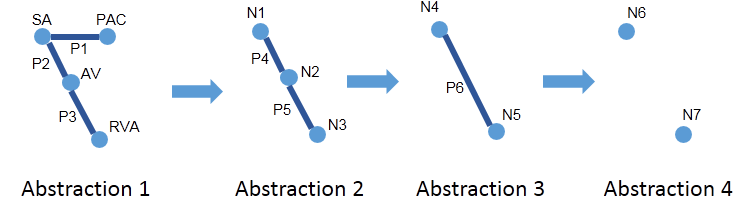
\includegraphics[width=0.9\textwidth]{figs/abs.png}
		%\vspace{-5pt}
		\caption{\small Stroke Volume as a function of heart rate and AV interval}
		  %\vspace{-15pt}
		\label{fig:SV}
\end{figure}

\subsection{Heart Model Validation}
In \cite{VHM_proc} our heart models were validated by physicians. With the rule-based heart model abstraction, each abstract heart model can be validated using the following sequence:
\begin{enumerate}
	\item Validate the initial heart model (structure)
    \item Validate all the abstraction rules applied.
\end{enumerate}

\section{The Heart Modeling Tool Box}
In the toolbox we have 4 data structures: 
\begin{itemize}
	\item Heart models
    \item Physiological behaviors of the heart
    \item Abstraction rules for the heart
    \item Physiological requirements
\end{itemize}
The heart model structure have following fields:
\begin{itemize}
	\item Heart parameter sets
    \item Rules applied to the model
    \item Behavior set
\end{itemize}
Functions associated with the heart model:
\begin{itemize}
    \item Display
    \item Heart Model validation
\end{itemize}

\section{Requirement-Guided Heart Model Selection}
Closed-loop requirements are mostly \textbf{conditional}, meaning that it should hold under certain environmental condition. For example, the following requirement:\\
\textsf{R1: When the intrinsic activation in the atria and ventricles are both less than 100bpm, the ventricular rate is less than 100bpm}\\
The requirement constrains on the \textsf{Atrial.self} and \textsf{Vent.self}, and reason about \textsf{Vent.act}


\subsection{Rules for Heart Model Eligibility Check}

\begin{itemize}
	\item The behavior (or its renames) constrained in the condition of the requirement should not be abstracted with other behaviors in the heart model
    \item 
    
\end{itemize}

\begin{Verbatim}
function [status,message]=eligible(HM,Req)
	for all BehaveObj1 in Req.condition
    	for all the BehaveObj2 in HM.behavior
        	while (BehaveObj1 not in BehaveObj2)||(BehaveObj2 not rename of BehaveObj1)
            	if 
\end{Verbatim}

\subsection{Example}
We perform \textsf{eligible(HM4,R1)} and the check fails, since \textsf{Atrial.self=N1.self=N4.self$\in$N6.self}. The check also suggest that \textsf{N3.self} and \textsf{P6.cond} should be seperated. If we go to HM3 and \textsf{eligible(HM3,R1)} is successful. So HM3 is the suggested heart model for requirement \textsf{R1}.

% ---- Bibliography ----
%
\bibliographystyle{unsrt}
{ \small 
\bibliography{bibliography}
}
\end{document}